\documentclass[letterpaper,twocolumn,10pt]{article}
\usepackage{epsfig}
\usepackage[mathscr]{eucal}
\usepackage{paralist}
\usepackage[T1]{fontenc}
\usepackage{caption}
\usepackage{subcaption}
\usepackage[font=small,labelfont=bf]{caption}
\usepackage{graphicx} 
\usepackage{xcolor} 
\usepackage{multirow} 
\usepackage{amsfonts}
\begin{document}

%don't want date printed
\date{}

%make title bold and 14 pt font (Latex default is non-bold, 16 pt)
\title{\Large \bf An Open Privacy Stack for the Web : Priv.ly }

%for single author (just remove % characters)
\author{
{\rm Sean McGregor }\\
Privly Foundation
\and
{\rm Carlos Jensen}\\
Oregon State University
\and
{\rm Jen Davidson}
% copy the following lines to add more authors
% \and
% {\rm Name}\\
%Name Institution
} % end author

\maketitle

% Use the following at camera-ready time to suppress page numbers.
% Comment it out when you first submit the paper for review.
\thispagestyle{empty}


\subsection*{Abstract}
Much work has been undertaken to add privacy to web applications, but
these works typically target a single use case and fail to generalize for all
web standards based applications.

In this paper, we present a web application stack that fixes web application privacy 
properties by means of a generalized ``injectable'' architecture. The application injection paradigm provides
for the implementation of many-to-any privacy applications-- whereby many different privacy applications can be integrated with any web-standard application.

We implemented the system with proof-of-concept browser extensions, 
but also show an optional method for extension-less operation. Several injectable applications are also presented in the context of
shared and distinctive threat models. 
Current injectable applications include libraries for symmetric key and public key cryptography, 
as well as functionality for a personal semantic datastore and information visualization.
A usability analysis of the approach is also presented.





\section{Introduction}

Online Service Providers (OSPs) like Facebook, Google, and Twitter help 
users create communities around their content and communications. 
Since, with rare exception, these communities are centralized and hosted by
a third parties, their usage tends to come with significant privacy costs:
\begin{enumerate}
  \setlength{\itemsep}{1pt}
  \setlength{\parskip}{0pt}
  \setlength{\parsep}{1pt}
  \item OSPs can be forced to turn over protected content without the users knowledge or consent~\cite{Greenwald2013}.
  \item OSPs subject content to continually changing permission structures and 
  system capabilities, which results in accidental leaks of information~\cite{Boyd2008}.
  \item Even sophisticated web technology companies have security vulnerabilities 
  that compromise billions of user messages~\cite{Symantec2011,Wee2011,Greenwald2013}.
  \item Content posted to OSPs is often subject to onerous terms and conditions~\cite{Gardner2011,Erwin2012,Unhosted2013}.
  \item Countries without strong press freedoms regularly censor content~\cite{MacKinnon2009,AssociatedPress2012}.
\end{enumerate}

User outrage surrounding a series of privacy imbroglios~\cite{Boyd2008} at 
Facebook shows that users care about online privacy, but Facebook's continued growth~\cite{Facebook2013} despite privacy issues 
indicates that users do not have a viable alternative. Existing alternatives 
suffer from the impediments of \begin{inparaenum}[\itshape a\upshape)]
\item \emph{Specificity:} the method solves a particular privacy issue, 
but fails to generalize to multiple use cases, or
\item \emph{Bootstrapping:} The communities never achieve the critical mass 
needed to compel non-privacy conscious users to adopt the method.
\end{inparaenum} 

We posit that any solution seeking to have a meaningful and significant impact in
 returning control over content to users needs to
\begin{inparaenum}[\itshape a\upshape)]
\item adapt to multiple use cases and web applications; and
\item fail gracefully by working without the need of any specialized client code.
\end{inparaenum} In this paper we propose Priv.ly as a flexible privacy stack
 meeting the adaptability and graceful failure requirements. Priv.ly provides a method for seamlessly viewing 
 content within the context of OSP applications while not permitting the OSP access
  to the content.

Priv.ly meets these requirements with a many-to-any
scheme, whereby \emph{many} different privacy applications can be embedded inside
\emph{any} website. The privacy applications provide \emph{adaptability} by supporting any web-implementable privacy application. 
Since the underlying privacy application is web based, a hosted fallback is employed to allow
for applications to \emph{fail gracefully}.
  
The Priv.ly threat model considers OSPs to potentially be adversarial and to have full control over the data presented inside the OSP's scripting environment. 
This allows OSPs to impersonate users, change user content, destroy user content, or leak data to 
third parties. Furthermore, OSPs can remove, restrict access to, or modify content 
once posted. We also consider governments and ill-willed users to potentially be 
adversarial, and capable of either colluding with the OSP or exploiting 
vulnerabilities in the OSP itself. The degree to which these problems are
mitigated or avoided is specific to the privacy application running on Priv.ly.
Priv.ly has a separate scripting environment viewable within the OSP's user 
interface which the OSP cannot inspect or alter.

We assume that the browser has access to a secure transport protocol in all 
communications. Further, we assume that the user's browser is not compromised.

Properly characterizing content privacy in the context of Priv.ly requires
specifying the privacy application that Priv.ly is running. Consequently, the
assumptions and strengths of several privacy applications are outlined
where specific applications are introduced.

This paper is organized as follows. We start with a discussion of the relevant related work. Next we detail the system's architecture in section
\ref{sec:privly_architecture} before outlining how multiple use cases may be 
satisfied by the architecture in section \ref{sec:privly_subsumed_use_cases}. Finally, we 
give a threat analysis in section \ref{sec:privly_security_analyses} and discuss an 
implementation in section \ref{sec:privly_implementation}.




\section{Related Work} \label{sec:related_work}

Since Priv.ly's motivation is to provide a suitable architecture for a large number of
privacy use cases, we highlight related works in this section as inspiration for Priv.ly.
Subsequent sections discuss these systems in the context of Priv.ly's architecture and 
introduce additional systems whose use cases are covered by Priv.ly.

Several privacy-preserving architectures have been proposed to replace successful 
web applications. Cristofaro et al.~\cite{Cristofaro2012} propose Hummingbird as a 
Twitter.com-like microblogging service that protects contents and hash tags from 
its centralized server. Two Facebook replacement services, EASiER 
\cite{Jahid2011} and Persona~\cite{Starin2009},
use attribute-based encryption to cryptographically enforce authorization.
While Hummingbird, Persona, and EASiER all maintain core elements of the social networks they 
aim to replace, they do not have a way to \emph{bootstrap} a user 
community beyond privacy-concerned users. Incumbency and the strength of the 
advertising model makes promotion of these privacy-preserving architectures challenging.

Distributed social networks do not require a profitable central provider because anyone can host content 
within the network. Nilizadeh et al.~\cite{Nilizadeh2012} proposed Cachet as a 
decentralized architecture for privacy preserving social networking, but the 
experiences of the Diaspora project indicate that Cachet is likely dead on arrival 
due to adoption issues. The Diaspora project built a user-owned distributed 
social network boasting 369,000 users~\cite{Diasp.eu2013}, but this is only 
0.04 percent of Facebook's total user base~\cite{Facebook2013}. The Diaspora 
project was an early innovator of asymmetric sharing, but the subsequent adoption 
of the approach by the Google+ social network removed Diaspora's competitive 
advantage and made it difficult for Diaspora to \emph{bootstrap} a community. 
In part to avoid needing to create a new community, Priv.ly builds on 
top of any web-standard infrastructure, which makes it possible to conscript the 
systems of entrenched OSPs.

flyByNight~\cite{Lucas2008} attempted to use Facebook's application infrastructure to create a
privacy application inside Facebook. flyByNight introduces a 
potential for ``legal privacy protection'' in the United States, which means that Facebook is capable of reading
user content, but it is legally prohibited from doing so because the privacy software introduces 
a ``legal expectation'' of privacy. Since Facebook makes frequent changes to their APIs,
the flyByNight system has likely been broken several times.
The flyByNight system also does not extend outside Facebook.

VPSN~\cite{Conti2011} and NOYB~\cite{Guha2008} protect Facebook profile information by means of browser extensions.
The VSPN browser extension replaces placeholder strings and photographs with their references file which is transmitted to other users via XMPP.
NOYB has a similar scheme where decryption keys are transmitted out-of-band.

Two systems at the extremes of usability and security are the paradigm Confidentiality as a Service (CaaS)~\cite{Fahl2012b} 
and the hyperlink-based cryptography of the browser extension 
Scramble!~\cite{Beato2011}. Fahl et al.~\cite{Fahl2012b} proposed CaaS as a means 
of increasing the usability of cryptographic systems. Content is shared with other 
OSP users through a ciphertext string, which is keyed by an unaffiliated CaaS 
provider. The CaaS provider performs cryptographic services on behalf of the user 
and protects the user from key loss. In order to gain access to content, an 
adversary would need to gain access to both the CaaS provider's keys and the OSP's 
ciphertext. However, there are no protections from the collusion of the CaaS 
provider and OSP.

A proof-of-concept implementation of the CaaS paradigm called 
TrustSplit~\cite{Fahl2012a} supports decryption of content on Facebook, and the 
developers manually add support for additional large social networks. When 
evaluated against our two criteria for success, TrustSplit proves to be an 
overly \emph{specific} solution that currently requires customization to adapt to individual 
websites. CaaS is also not generalized to support
multiple privacy applications.

Scramble!~\cite{Beato2011} eschews the use of third parties for key sharing and instead relies on public key cryptography. 
Scramble is a Firefox extension that allows users to cryptographically enforce
access control lists (ACL) defined locally in the browser extension.
The ciphertext is stored on a content server, referenced by a hyperlink shared via 
the OSP. The extension-resident public key cryptography means that users cannot 
encrypt content for users who have not generated and pushed a public key 
(\emph{bootstrap} problem). Scramble also relies on the user to manage their ACL, 
which poses usability challenges~\cite{Fahl2012}. Scramble works more 
effectively on multiple websites than TrustSplit, but it is still confined
to a single privacy application, cryptography scheme, and key manager.

Neither Scramble nor TrustSplit protect the plaintext from OSPs \emph{after} it is 
decrypted. TrustSplit and Scramble place the content directly onto the OSP's 
scripting environment, which an adversarial OSP could use to send all decrypted 
content back to the OSP thereby making the encryption meaningless. Priv.ly injects 
content within an HTML iframe element, which the host page does not have access to 
due to the Same Origin Policy~\cite{Barth2009}.

CaaS emphasizes usability as compared to Scramble~\cite{Fahl2012b}, but Scramble 
offers stronger security guarantees by storing the keys locally. Priv.ly supports 
both the usability of CaaS and the security of Scramble from a single codebase by 
abstracting the components of both models into an application stack.

\section{The Web Privacy Stack: Priv.ly} \label{sec:privly_architecture}

Every website has its own navigation structure, layout, and audience, but when 
you strip away these unique attributes of websites, you are left with data-- chats, 
emails, photos-- that can be treated uniformly across all websites. Operations on 
these data like encryption and signing, can be performed with indifference to their 
context and their contents.

Priv.ly uses data indifference to create the notion of ``Injectable Applications,'' 
which are full web applications that are injected into the context of other web 
applications. Since these applications are scoped to data and not layout, their 
properties are simplified and usable across the web.

Priv.ly works within browser extensions by scanning web pages for specially 
formatted hyperlinks. When the extension detects the hyperlink, it ``injects'' 
the link into an iframe that is served locally from the browser extension. 
Since the injected application is a full web application, the app could 
potentially support any web-implementable feature.

\begin{table}
    \begin{tabular}{|p{2.5cm}|p{4.5cm}|}
        \hline
        \textbf{Name}                  & \textbf{Description}                                                                                             \\ \hline
        Host Page \newline(Host-P)              & A rendered web application from an Online Service Provider, viewed on the client.                                             \\ \hline
        Content Link \newline(C-Link)           & The URL for the hosted version of the application, and the parameters required for the application.                      \\ \hline
        Extension \newline(Extension)              & The packaged code and user interface changing the behavior of the user's browser.                       \\ \hline
        Injectable Application \newline(Injectable-App) & The application referenced by the C-Link. This application is viewed in the context of the Host-P, but the Host-P does not have access to the HTML or scripting environment.                                                       \\ \hline
        Content Server \newline(C-Server)         & A server hosting plaintext, ciphertext, keys, or other content required by the Injectable-Apps.
    \end{tabular}
    \caption{Definitions for components of the Priv.ly Application Stack}
    \label{tab:definitions}
\end{table}

We introduce system definitions in Table \ref{tab:definitions}. Instead of 
adhering to Scramble's limit of a single public key infrastructure scheme, the 
URL format is generalized as a Content Link (C-Link) to support web application 
selection and parameters. The C-Link parameters define application options and 
data endpoints for an Injectable Application (Injectable-App), which is a full 
web-application that can be viewed in the context of an OSP's Host Page (Host-P). 
When users have the Priv.ly browser extension (Extension) installed, they benefit 
from a more seamless user experience and added security guarantees. If users 
do not have the extension installed, they can expect to use the Injectable-App 
code served by a content server (C-Server) referenced in the domain of the C-Link.

The processes involved in generating and reading 
content when a Priv.ly Extension is installed are outlined below.

\subsection{Processes} \label{sec:privly_processes}

\subsubsection{Posting Content}

\begin{center}
  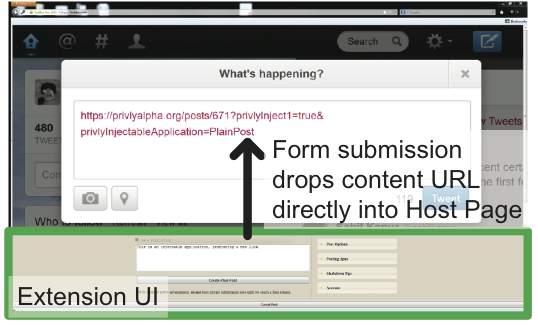
\includegraphics[height=44mm]{graphics/Posting-Process-Twitter.eps}
  \captionof{figure}{User interface for generating a new C-Link for Twitter on the Firefox 
  Extension. The Extension's form at the bottom of the browser is visually separated 
  from the Host-P above it, and is seeded with the content found on the Host-P.}
  \label{fig:posting-process-twitter}
\end{center}

\begin{center}
  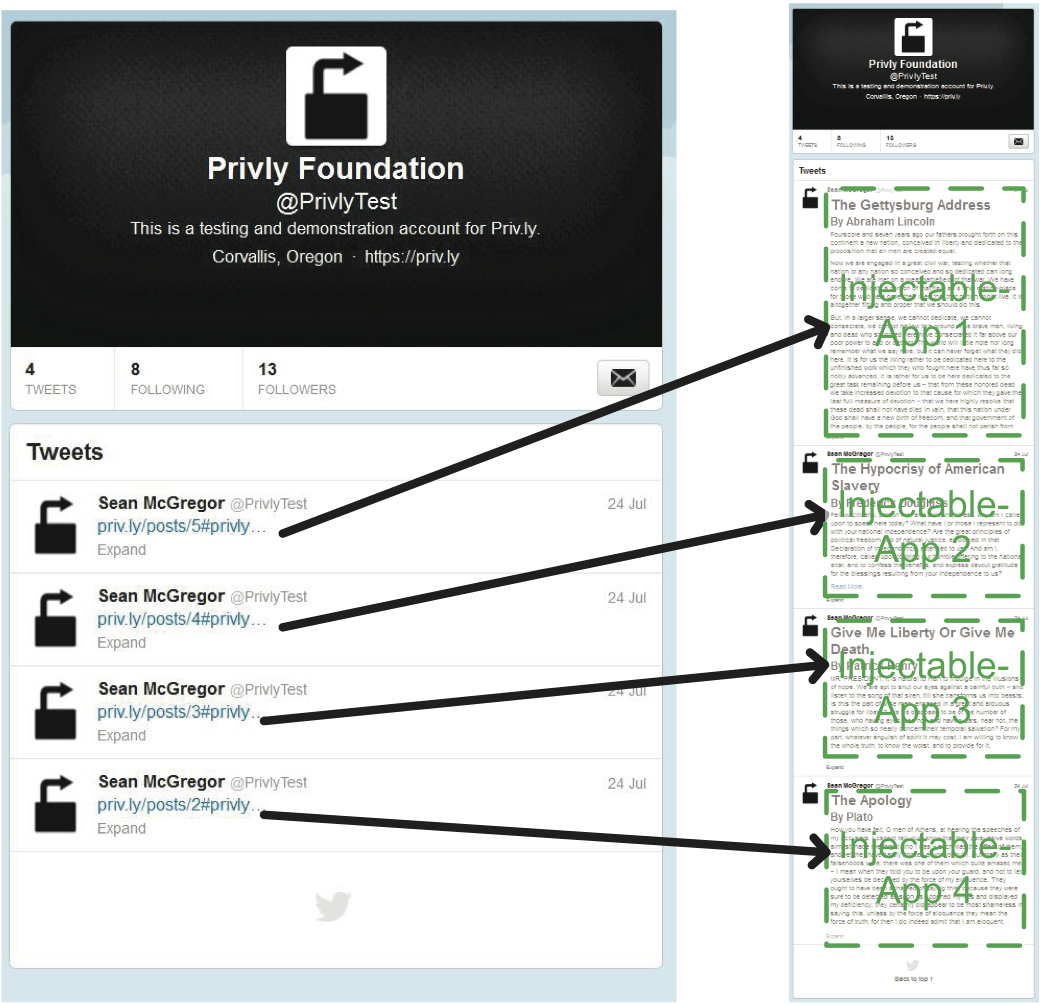
\includegraphics[height=70mm]{graphics/Reading-Process-Twitter.eps}
  \captionof{figure}{Twitter.com before and after content is injected. The green boxes 
  indicate regions that have a separate scripting environment from the rest of the 
  page. The injection of content allows for ``tweets'' longer than 140 
  characters.}
  \label{fig:reading-process-twitter}
\end{center}

Here we present a generalized process by which protected 
content is posted to a Host-P. We present a generalized process because it makes use of all
potential communications channels between the system's components. Some Injectable-Apps will 
not communicate with the C-Server.
The process can be as transparent to the user as 
desired, or it can be made more automatic by performing all operations in the 
background and working exclusively with the form elements of the Host-P.

\begin{compactenum}
  \item The user initiates the posting process through an Extension context 
  menu\footnote{A context menu is usually displayed after right-clicking content 
  on a web page.} or keyboard shortcut. The user then types content into an 
  Injectable-App as shown in Figure \ref{fig:posting-process-twitter}.
  \item The user submits the Injectable-App's form.
  \item The Injectable-App optionally encrypts the data with its encryption scheme.
  \item The Injectable-App sends a JSON object containing the encrypted data to the C-Server.
  \item The C-Server returns the C-Link to the Injectable-App.
  \item The Injectable-App modifies the C-Link and passes it to the Extension.
  \item The Extension places the C-Link on the Host-P where the context menu 
  started the process.
\end{compactenum}

\subsubsection{Reading Content}

Here we present the reading process for Priv.ly 
content, in which C-Links are seamlessly ``injected'' so that their referenced 
content is fetched, processed, and displayed in the context of the Host-P.
Again we present a generalized view of the operations that the Injectable-App
are likely to undertake. Specific applications will be presented below.

\begin{compactenum}
  \item The Extension adds a JavaScript to the Host-P that watches for a C-Link.
  \item The Host-P JavaScript discovers a C-Link and 
  injects a hidden Injectable-App in an iframe next to the C-Link.
  \item The Injectable-App requests content from the C-Server linked by the 
  C-Link.
  \item The C-Server returns JSON to the Injectable-App.
  \item The Injectable-App decrypts the content and displays it.
  \item The Injectable-App sends the desired height of its iframe to the script 
  added to the Host-P in step 1. The Host-P script can then resize the iframe to 
  match the content. The original C-Link is hidden, and the Injectable-App is 
  displayed on the Host-P.
\end{compactenum}

\subsection{Component Discussion}

\subsubsection{Host Page} \label{sec:privly_content_script}

Host pages are modified by means of content scripts that are added by the browser
extension but potentially modified by the Host-P's scripting environment.

Priv.ly treats the Host-P as indifferent to Priv.ly operation, but a potential 
adversary to content security. Although unaffiliated developers may wish to engage 
in cat-and-mouse games with antagonistic Host-Ps, Priv.ly takes the view that most 
OSPs value a user's time-on-site more than access to cleartext content. If the 
Host-P forces the user to click through to Priv.ly content instead of allowing for injection, they effectively reduce 
time-on-site and potential advertising revenue.

The Injectable-App may want to expose an API to the Host-P for 
content styling or other presentation concerns~\cite{Barth2009,Jackson2007}. If a 
particular Injectable-App is well integrated with the Host-P, then it could 
conceivably be ``recommended'' by the OSP.

\subsubsection{Extension} \label{sec:privly_extension}

The Extension provides the user interface, and acts as the gatekeeper between the 
untrusted Host-P and trusted local code.

All browsers maintain a clear visual separation between Host-P content and browser 
user interface elements, like the address bar. Without the visual separation, a 
user is vulnerable to spoofing attacks, which is when the Host-P tricks the user 
into believing they are on a trusted website. 

Extensions can access user interface elements not available to web applications, 
which allows users to trust extension functionality presented next to an unsafe 
Host-P. The example posting screen capture in Figure 
\ref{fig:posting-process-twitter} shows a frame displayed outside the Host-P that 
accepts user content. The Extension opens the application for generating a new 
C-Link, and manages the interface between the application and the Host-P.

Browser extensions are usually built on top of web standard technology like
HTML and JavaScript, but their architectures have no shared standards. Essential APIs
often have eccentricities requiring platform-specific programming. To harmonize the
many differences between extension APIs, Priv.ly provides a shared set of 
libraries to the Injectable-Apps that hides the inconsistencies from developers.
For example, the localStorage API is not available on Firefox extensions, but there
is database support and a basic key-value storage mechanism for preferences.
JavaScript adapters available to all Injectable-Apps harmonizes these different
APIs.

When an Injectable-App is injected by a browser extension, it has API access to the
data managed by the Extension, including any key databases required by Injectable-Apps.
This shared storage allows different Injectable-Apps to implement key managers, or use the
keys defined by another key manager.

\subsubsection{Content Link}

Several objectives are achieved by tying Host-P integration to specially formatted
URLs. First and foremost, it provides a 
fallback for users who do not have the Extension running on their browser. Unlike 
methods where non-link ciphertext is placed into the Host-P, the user can click 
the link to learn about the content type. If the C-Server stores plaintext, or has 
access to the decryption keys, the user could view the content without need for a 
local extension.

It should be noted that W3 
standards~\cite{Fielding1999} do not place any limit on the length of URIs. 
Further, the anchor text is not sent by the browser on HTTP requests. When 
combined, these standards permit placing keys, ciphertext, and signatures on the 
hyperlink's anchor without giving the C-Servers access.\footnote{The anchor text, 
also known as hash text, is not sent with HTTP requests. The web application 
returned by the request may include JavaScript code that sends the hash to an 
arbitrary server. Hence secret sharing via the anchor text is a compromise between 
usability and security.}

Injectable-Apps have access to all the parameters specified on both the parameter 
string and the anchor string. Several C-Link parameters specific to individual 
Injectable-Apps are covered in 
the context of their applications in section \ref{sec:privly_injectable_applications}.
Other types of parameters are covered in  Table \ref{tab:parameters}.
To simplify injectable link identification, the string ``PrivlyInject1'' is added 
to injectable URLs. This string is provided as an optimization to speed link 
injection, but it is not strictly necessary should the C-Server need to obfuscate 
its compatibility with an Injectable-App.

\begin{table*}
    \begin{tabular}{|l|l|p{10.8cm}|}
        \hline
        \textbf{Parameter}                   & \textbf{Component}              & \textbf{Purpose}                                                                                                                                                                                            \\ \hline
        PrivlyInject1               & Host-P              & Tags the C-Link as accepting injection.                                                                                                                                                      \\ \hline
        PrivlyApp & Extension & Selects the Injectable-App.                                                                                                                                                         \\ \hline
        PrivlyDataURL               & Injectable-App & Gives the URL of the data-only endpoint for the content. Injectable-App parameters are specific to the app specified in the PrivlyApp parameter, so this parameter is not always used.                                                                                                                                           \\ \hline
    \end{tabular}
    \caption{Parameters found on the C-Link for influencing the operation of link injection and Injectable-App operation.}
    \label{tab:parameters}
\end{table*}

The parameter ``PrivlyApp'' may be specified by the 
C-Link to indicate 
which Injectable-App should be served locally for the content.

\subsubsection{Content Server} \label{sec:privly_content_server}

The C-Servers host content intended for Injectable-Apps. In general they should 
present data-only endpoints, but in cases where users do not have the extension 
installed, they should present a fallback web application. The fallback application
is specified on either the URL's path or parameter string so the server can route
the request to the proper web application.

Currently implemented C-Servers provide serialized JSON storage as simple key-value 
pairs. This maximizes C-Server compatibility with current and future Injectable-Apps.
As noted earlier, a C-Server is not necessarily required by Injectable-apps that 
fully specify all their required data in the C-Link's parameter string or hash text.
However, a link to nowhere presents challenges in \emph{bootstrapping} a user comunity since
users will not know that the content is viewable when a browser Extension is installed.

Injectable-Apps using a C-Server allow for propogating content updates to anywhere the
C-Link has been shared.

\subsubsection{Injectable Applications} \label{sec:privly_injectable_applications}

Injectable-Apps are the primary abstraction of the Priv.ly architecture. They 
provide a means for writing and deploying new privacy concepts independent of 
Host-Ps. Although privacy use cases are Priv.ly's primary design consideration, 
Injectable-Apps could potentially support any web functionality, but more dynamic functionality increases the 
number of points at which content may be compromised. By limiting the operations 
the applications can perform, we can provide security guarantees for user data and 
cryptographic identities.

Injected applications are not permitted to execute remote code, so content must 
be delivered on a data-only endpoint, or be subject to strong HTML sanitization and
sandboxing. 
By packaging verified versions of the Priv.ly Injectable-Apps, Priv.ly prevents many 
potential issues with JavaScript security and clickjacking~\cite{Huang2012}.

Injectable-Apps may optionally support any web-implementable cryptosystem
that matches the application's threat model.
In cases where the transport protocol and the C-Server are 
both trusted, content level cryptography may not be necessary. This 
functionality has been implemented as the Injectable-App PlainPost.

Symmetric keys specific to individual links 
may be safely processed in JavaScript. One interesting application of JavaScript 
cryptography used by Priv.ly is implemented in the ZeroBin~\cite{Sebsauvage2013} 
Injectable-App. ZeroBin uses 256 bits AES to encrypt content before sending the 
ciphertext to a C-Server. The C-Server then returns a C-Link to the 
Injectable-App, which adds the key to the anchor text of the C-Link before sharing 
it over an OSP. This arrangement neatly mirrors the CaaS paradigm in that 
decryption requires access to both the Host-P and the C-Server.

Rolling out an injectable application with public key cryptography raises 
questions of how to establish identities for people who have not yet published a 
public key. As a stopgap measure, a scheme similar to Mozilla's 
Persona~\cite{Mozilla.org2013}
may be employed, where a trusted authority temporarily holds keys until such time 
that a user generates their own, and invalidates the trusted authority. Much existing
work on usable key distribution is compatible with Priv.ly~\cite{Beato2011,LeapEncryptionAccessProject2013}, but a full exploration of
this topic is beyond the scope of this paper.

We should note that the flexibility of Injectable-Apps 
extends to the management of trust in keys. Multiple key managers can coexist in Priv.ly. 
Thus different users can decide which Injectable-App key managers are appropriate for
their use cases. If users prefer to manually import and audit
their keys, then they can use a key manager that mimics the user interface of 
established systems like the GPG command line interface~\cite{Project2013}. 
Since most users have difficulty with the traditional way of managing keys~\cite{Fahl2012,Whitten1999}
new key managers will be introduced in subsequent works.

Seven Injectable-Apps are currently under development. These ``starter apps'' form
the foundation upon which more complex applications can be built. They range from
the simplistic ``PlainPost'' application that uses no content cryptography, to
a proof-of-concept implementation of PGP. Each application will be introduced in
more depth in the context of discussing application-specific properties in section \ref{sec:injectable_apps}.

\section{Baking Privacy Applications in Priv.ly} \label{sec:privly_subsumed_use_cases}

Priv.ly's ability to implement prior work in the form of Injectable-Apps is how we 
evaluate the effectiveness of the application stack. When building these 
approaches on Priv.ly, they should be viewed in the context of security analysis of 
their original implementation, as well as Priv.ly's analysis found in section 
\ref{sec:privly_security_analyses}.

Several approaches require their own Injectable-App within the Priv.ly stack. 
Scramble~\cite{Beato2011} and TrustSplit~\cite{Fahl2012a} could be implemented as Injectable-Apps.
Persona, EASiER, and Hummingbird could all be seamlessly implemented on top of existing social networks
using Injectable-Apps that target their use case.

The browser extensions for VPSN~\cite{Conti2011} and NOYB~\cite{Guha2008}-- which protect Facebook profile information-- are both implementable as their own Injectable-App.
Further, if users have different privacy expectations for different parts of their profile, then they could protect different parts of their profile with different Injectable-Apps.

Priv.ly's app infrastructure establishes a similar ``legal privacy protection'' as flyByNight. 
If a user hosts their content on their own server or a server with a privacy centered terms of service,
then they likely will have met the appropriate legal test for expectation of privacy in the United States.

Decentralized architectures like Diaspora could serve as C-Servers for the Priv.ly 
stack. The C-Link could provide an effective method for cross-posting content to 
other social networks, thereby \emph{bootstrapping} the Diaspora community while 
maintaining privacy.

The OTR~\cite{Goldberg} and PGP~\cite{garfinkel1994pgp} protocols are explored in section
\ref{sec:injectable_apps} along with several other Injectable-Apps.


\section{Threat Analyses} \label{sec:privly_security_analyses}

This section concentrates on distinctive threats of Priv.ly's injectable
architecture. Threats to the communication channel~\cite{Goodin2013} and C-Server have been well
documented~\cite{Goodin2013a} so these analyses focus on concerns unique to injecting applications into untrusted web applications. 

\subsection{Spoofing} \label{sec:privly_spoofing}

When content is modified or injected by a browser extension, the resulting content 
may break the visual separation between user-submitted content and site 
navigation. This creates a potential vector for users to craft spoofing attacks, 
which may lead a user to install malware or divulge sensitive information, 
including credentials for the Host-P.

To combat spoofing, the separate scripting environment of the Injectable-App 
displays a custom tooltip, as shown in Figure \ref{fig:gylph}, indicating the source and type of content. The tooltip 
appears when the user hovers their cursor over the content.


\begin{center}
  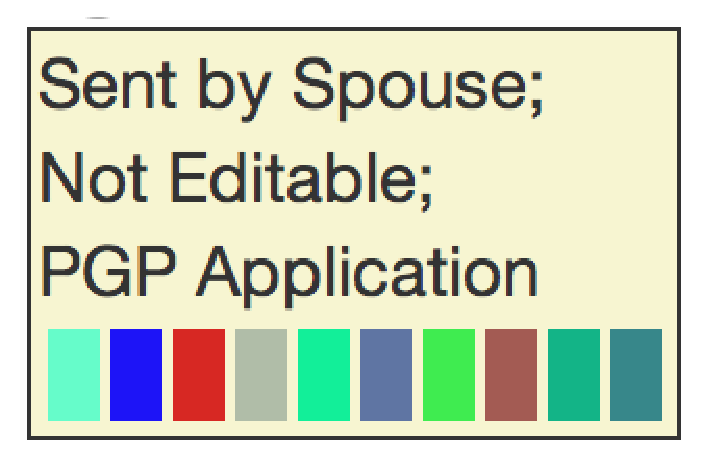
\includegraphics[height=25mm]{graphics/glyph.eps}
  \captionof{figure}{Contextual anti-spoofing tooltip. The sequence of colors is randomly generated on each of the extensions.}
  \label{fig:gylph}
\end{center}

A second type of spoofing may occur if the Host-P attempts to present its content 
as originating from an Injectable-App. Priv.ly content does not benefit from the 
guarantees provided by the browser address bar, so it must provide a method for 
verifying the origin of Injectable-Apps within the context of an untrusted Host-P. 
To authenticate the tooltip, a unique random glyph (Figure \ref{fig:gylph}) is associated with every 
Extension. The glyph is displayed next to the tooltip of injected applications.

Other services attempt to handle verification by shifting the color of 
content~\cite{Fahl2012b}, or offer no guarantees on the origin of data when 
injected~\cite{Beato2011}.

\subsection{Host-P Knows Content Length}

The Same Origin Policy requires Injectable-Apps to tell the extension the desired 
height of their iframe. When the iframe is resized in response, the Host-P can 
determine whether content exists and the user has access by monitoring the height 
of injected iframes and reporting back to the OSP via an asynchronous JavaScript request.

\subsection{User Understanding}

Priv.ly multiplies the usability challenges inherent in cryptographic 
systems~\cite{Whitten1999,Fahl2012} by providing for multiple Injectable-Apps. The non-profit foundation managing Priv.ly development mitigates this concern by enforcing 
consistent design and dissemination of system concepts, however communicating 
system concepts effectively remains a challenging problem.

The risks inherent in publishing a set of cryptographic applications requires an understanding that many users have limited knowledge of cryptography. Injectable-Apps must 
pass security assessments, as well as an evaluation of the non-technical 
user's understanding of the concepts. Technical users can be afforded complete 
freedom in the operation of Priv.ly, including using untested Injectable-Apps, but 
non-technical users may not.

The Haystack system's early rollout provides a model for how not to publish new 
cryptographic applications. Haystack promoted to users who could potentially be 
targeted by their government for their political activities before their approach 
was public and reviewed. Subsequent review revealed that governments could easily 
compromise Haystack data~\cite{Arthur2010}.

\subsection{Priv.ly Blocking}

While some OSPs would undoubtedly block Priv.ly, it is our belief that the majority 
of sites would rather permit Priv.ly operation than potentially lose users. In the event that independent developers wish to force 
integration with an unwilling Host-P, there are several options.

Significant progress has been made in adding steganography to encrypted content. 
Steganography refers to concealing a message within another message. A browser extension named FaceCloak 
introduced steganography and cryptography by posting 
random Wikipedia sentences to Facebook. Another extension, For Some Eyes 
Only~\cite{F.BeatoI.IonS.CapkunM.Langheinrich2013} generalized FaceCloak's 
approach by using Scramble! as a base implementation. Instead of posting a link to 
the host page, For Some Eyes Only generates a plain English sentence that serves 
as an index for discovering the content's URL. For Some Eyes Only, and 
steganographic solutions in general, still have serious challenges in 
usability~\cite{F.BeatoI.IonS.CapkunM.Langheinrich2013}.

While steganography could be built on top of the Priv.ly stack by modifying the 
script added to the Host-P, steganographic approaches are not included in Priv.ly because they are untenable without deactivating Host-P JavaScript. 

Instead of promoting a cat-and-mouse game, Priv.ly's main development branch
explicitly allows for Host-Ps to disable extension 
operation through a custom attribute on the body tag of HTML documents. Only 
through mass adoption of the Priv.ly system will it become clear whether OSPs 
accept the trade of losing cleartext access for Priv.ly's hypothesized increase in time-on-site. Until Priv.ly is adopted by a large proportion of a site's user base, OSPs
are unlikely to modify their HTML to deactivate Priv.ly injection.

Future development may also allow for the Host-P to influence the operation of 
Injectable-Apps so that they maintain the core elements of their user community. 
For instance, Twitter.com may want to limit the display of Injectable-Apps to 140 
characters to stay consistent with the non-extended user experience. We do not 
consider Host-P influence to be a system threat so long as its only result is 
better usability.

\subsection{Other Extensions}

Browser extensions typically have more privileged access to the browser than 
Host-P applications~\cite{Bandhakavi2011,Carlini2012}. Extensions pose challenges 
to the security of the user's private key that are just as severe as a compromise 
of the entire system. In some cases, it may be possible for the Priv.ly extension 
to warn against installing lesser known extensions. Until extension sandboxing is 
strictly enforced in the browser the best defense is to avoid potentially 
dangerous extensions.

\subsection{Tracking}

The unique identity of the C-Link combined with selective posting to a Host-P has 
the power to track user page views across the internet. For instance, a user with 
a malicious C-Server could email a C-Link to someone and log when and where the 
content was accessed.

Users may shield their location using systems like Tor~\cite{Dingledine2004}, but 
preventing the server from knowing whether content is accessed will not be achieved
until the C-Server is paired with an appropriate peer-to-peer strategy. This
``access obfuscation'' will be a focus of future work.

Priv.ly reduces the risk of tracking by malicious servers by providing an editable whitelist 
of trusted domains that abide by privacy rules consistent with user expectations. 

This threat does not apply to Injectable-Apps that don't use a C-Server for
content.

\subsubsection{Distributed Denial of Service (DDoS)}

A website could generate thousands of requests for a whitelisted server by placing 
Priv.ly-type links in a portion of the page that is not visible to the user. Priv.ly 
makes an effort to mitigate this threat by limiting the number of links a single 
page can inject to between 30 and 50, depending on the performance of the browser. 
Still, if Priv.ly is adopted by a large number of users, a comment on a high 
traffic site could overload nearly any C-Server. Further, when a user or Host-P 
re-shares a C-Link on a high-traffic site, even if visiting users don't have 
access to the content, they still generate a request to the server.

Several strategies could mitigate this threat, including individualized user DNS, 
building content servers on scalable infrastructure, and signing the scope of a 
link to a particular domain.

This threat does not apply to Injectable-Apps that don't use a C-Server for
C-Link specific content.

\section{Priv.ly Implementation} \label{sec:privly_implementation}

\subsection{Injectable Applications} \label{sec:injectable_apps}

The distinctive properties of Injectable-Apps make it difficult to simultaneously present them in a single analysis.
In the interest of space, we are choosing four particularly interesting sets of assumptions to highlight the differences between the current Injectable-Apps. 
We should note that these are not the only potential cases. We define the sets of assumptions as:
\begin{inparaenum}[\itshape a\upshape)]
\item the C-Server gives read-access to all its data (public);
\item the C-Server only gives read-access for a specifically requested C-Link (Trusted);
\item the C-Server only gives read-access if the requestor is explicitly authorized (Trusted Authenticating); or
\item the C-Server is compromised and the OSP does not share the C-Link unless a user is authorized via the OSP (Trusted OSP+Compromised C-Server).
\end{inparaenum} The final case flips the assumption from an adversarial OSP to a trusted OSP and a compromised C-Server. The first three
cases assume that the OSP may give its content to anyone.

Table \ref{tab:use_cases_served} lists the problems that an Injectable-App mitigates under these conditions when it displaces cleartext content on an OSP.
The Injectable-Apps follow:

\begin{table*}
    \begin{tabular}{|p{3.2cm}|p{2.5cm}|p{2.5cm}|p{2.5cm}|p{2.5cm}|}
        \hline
        \textbf{Injectable-App} & \textbf{Public C-Server} & \textbf{Trusted C-Server} & \textbf{Trusted Authenticating C-Server} & \textbf{Trusted OSP+Compromised C-Server}                                                                                                                                                                                              \\ \hline
        PlainPost               & 4                & 4         & 1,2,3,4,5  & -           \\ \hline
        ZeroBin and ZeroVis     & 4                & 4         & 1,2,3,4,5  & 1,2,3,4,5   \\ \hline
        PGP                     & 1,2,3,4,5        & 1,2,3,4,5 & 1,2,3,4,5  & 1,2,3,4,5   \\ \hline
        IRC                     & NA               & NA        & NA         & NA          \\ \hline
        OTR                     & NA               & NA        & NA         & NA          \\ \hline
        IndieData               & NA               & NA        & NA         & NA          \\ \hline
        \multicolumn{5}{|p{16.0cm}|}{
        {
          \footnotesize
          Mitigated:          
          \begin{enumerate}
          \setlength{\itemsep}{1pt}
          \setlength{\parskip}{0pt}
          \setlength{\parsep}{1pt}
          \item Cleartext is surrendered without user's knowledge or consent.
          \item Permissions on cleartext are retroactively modified.
          \item Vulnerability compromises content.
          \item Cleartext is subject to negative terms and conditions. 
          \item C-Link may be selectively censored on the OSP based on its cleartext.
      \end{enumerate}
      }
      } \\
      \hline
    \end{tabular}
    \caption{
    Table of mitigated problems. 
    Use cases are mitigated when it is unlikely to happen under the current assumptions. The columns assumptions are:
    (public) the C-Server gives read-access to all its data; (Trusted) the C-Server only gives read-access for a specifically requested C-Link;
    (Trusted Authenticating) the C-Server only gives read-access if the requestor is explicitly authorized; or
    (Trusted OSP+Compromised C-Server) the C-Server is compromised and the OSP does not share the C-Link unless a user is authorized via the OSP.
             }
    \label{tab:use_cases_served}
	
\end{table*}

\emph{PlainPost.}

The most basic application, PlainPost, 
displays text requested from a remote C-Server. It is the ``most universal app,''
since its only requirement is that the content be stored on a server. The data can be hosted anywhere because the application is backend agnostic. Since the
application does not use any cryptography, this application requires the use of
a C-Server and is thus necessarily vulnerable to DDoS and tracking if a peer-to-peer network is not employed.

\emph{Symmetric Cryptography: ZeroBin and ZeroVis.}

The ZeroBin~\cite{Sebsauvage2013} and ZeroVis Injectable-Apps 
build on PlainPost's foundation with symmetric key cryptography~\cite{Stark2009}. The key is 
shared on the anchor of the C-Link, which means that the content can be decrypted 
by permissioned users holding the C-Link regardless of whether they have the Extension installed.

These applications strike a compromise between usability 
and security to allow sharing when a user's social connections have not 
necessarily been \emph{bootstrapped} into Priv.ly. 
When a user has the extension installed, only parties with access to both the OSP and the C-Server can recover the cleartext since the C-Link's anchor text is never sent to the C-Server by the client.
When a user clicks the ZeroBin C-Link without the Extension installed, the C-Server can force access to the cleartext by sending the client a false version of the ZeroBin Injectable-App.
Although network effects dictates which social networks are useful for a user, a C-Server could conceivably be any person or company that the user trusts.

    \begin{figure*}
        \begin{center}
        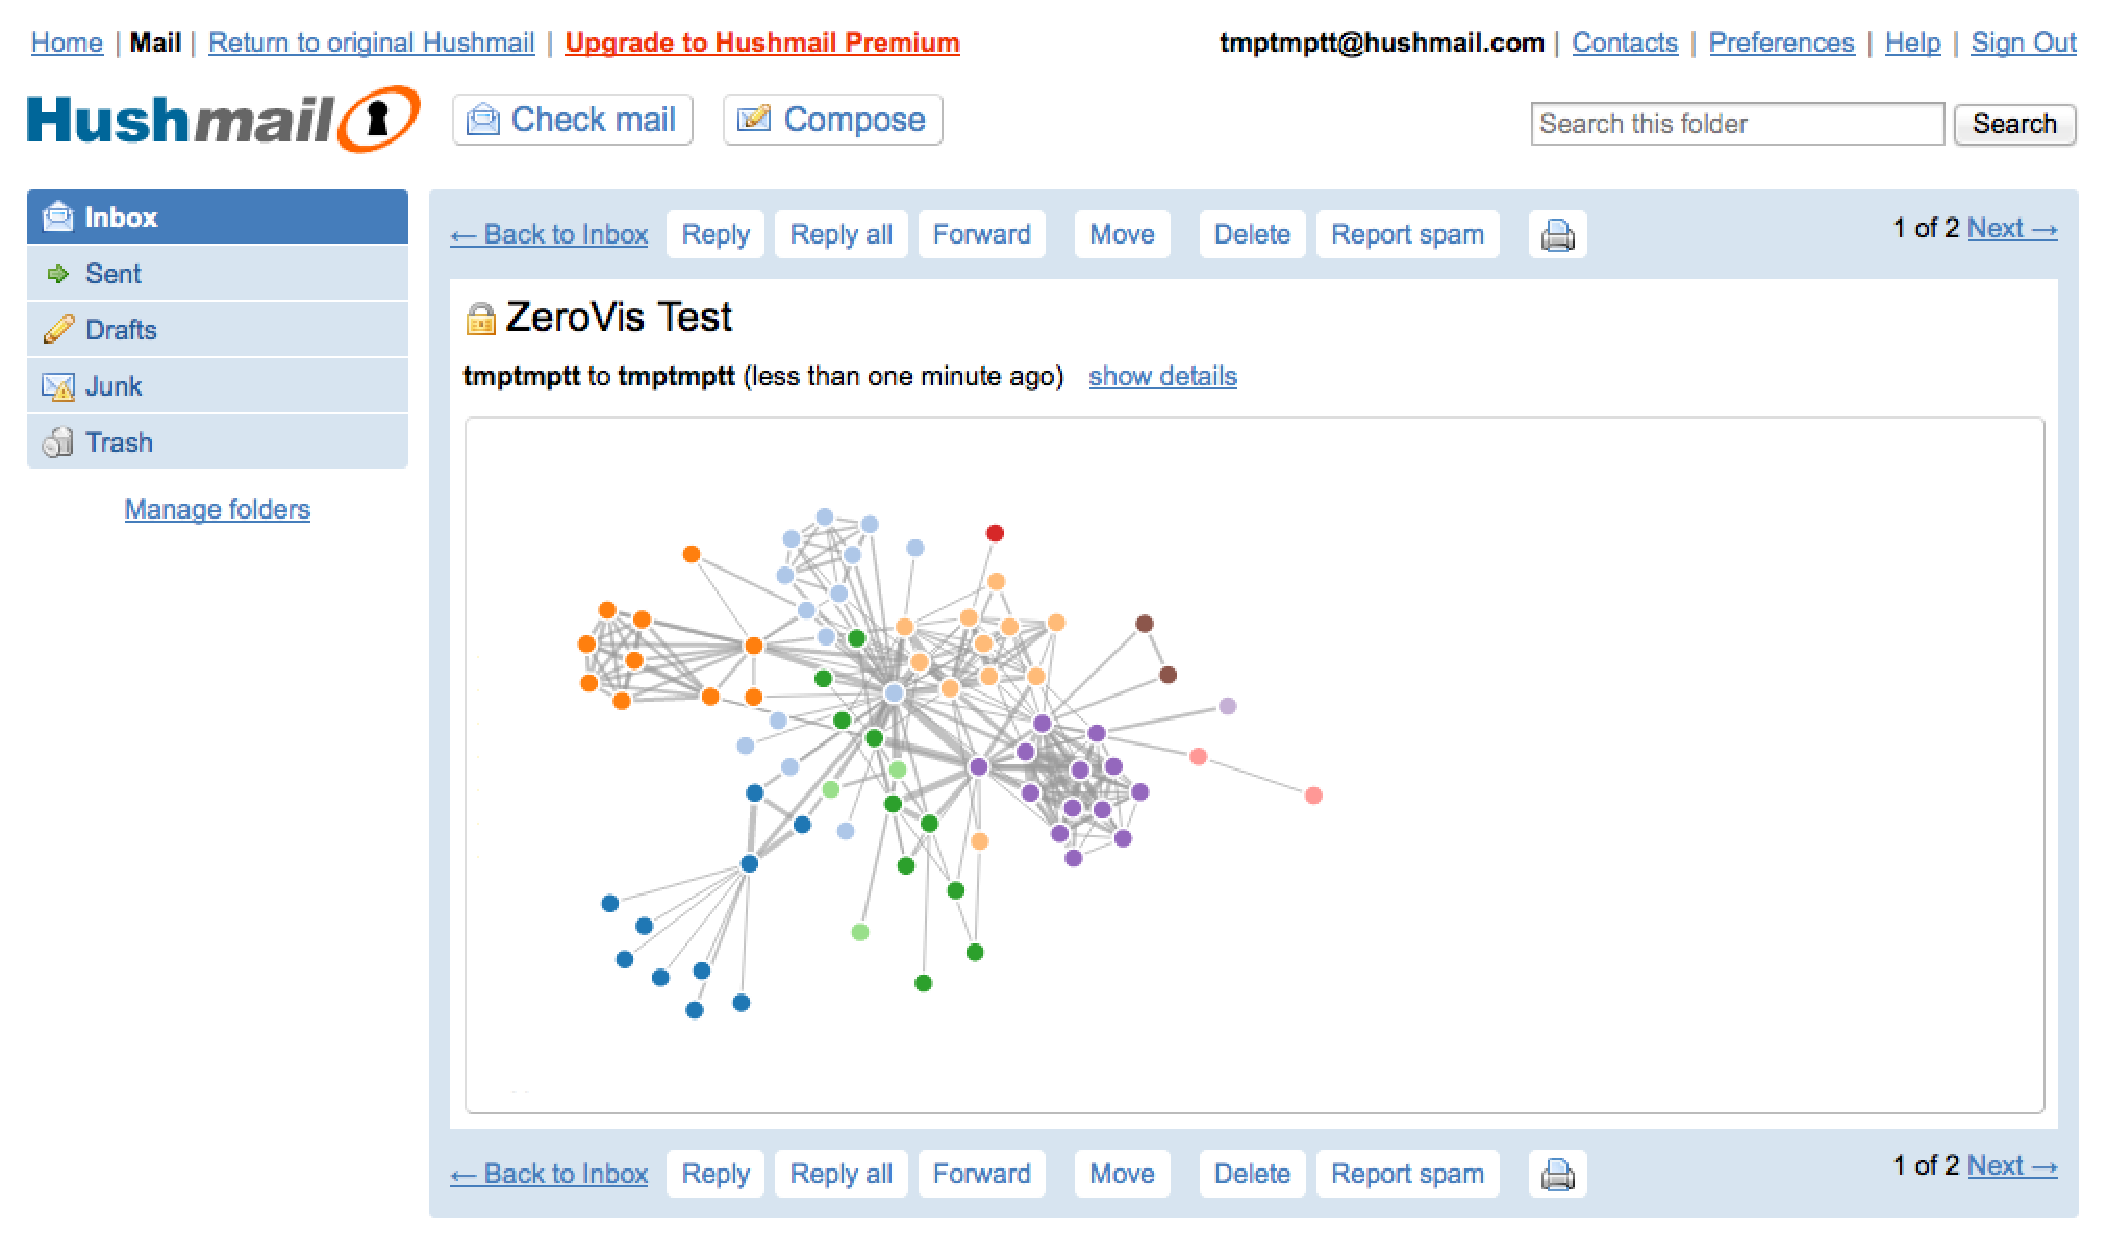
\includegraphics[height=70mm]{graphics/ZeroVisHushmail.eps}
        \captionof{figure}{A Priv.ly application featuring an interactive social graph visualization is injected into the notorious \cite{Singel2007} Hushmail web application. The content in the visualization is not accessible to Hushmail's scripting environment and the associated data is stored as encrypted and serialized data on the C-Server.}
        \label{fig:zerovis}
        \end{center}
        
    \end{figure*}

The ZeroVis Injectable-App builds on top of ZeroBin to provide a proof-of-concept application for information visualization of AES decrypted data. Figure \ref{fig:zerovis} shows ZeroVis's interactive social graph visualization injected into the context of a webmail provider. This application is provided as a demonstration of the flexibility of Priv.ly's approach and the capacity for enabling robust web-standard applications.

As Priv.ly gains more coverage in a user's social graph, we expect users to begin preferring sharing keys out-of-band or using public key cryptography.

\emph{PGP.}

The PGP application is currently a bare-bones application used for generating new keys, as well as encrypting and decrypting content. Developers are working on more usable key managers to pair with the application, but existing libraries focus on the traditional web-of-trust~\cite{garfinkel1994pgp} model that is not sufficiently usable for a less technical user base~\cite{Whitten1999,Fahl2012}. The focus of key distribution development is a forthcoming method leveraging the Extension to distribute a consensus model via a user's web interactions. This will allow the Priv.ly architecture to leverage the de facto identity system of the web: social networks and email. While there is great potential in developing new key management systems for Priv.ly, we will publish this Injectable-App with a ``traditional'' key manager before pushing out novel designs since the Injectable-App architecture can support multiple key managers.

It should be noted that key exposure should be mitigated by adding an additional symmetric key to the process that encrypts the whole PGP ciphertext. The additional key is then bound to the C-Link on the Host-P in the same way that ZeroBins store their symmetric key. The additional key means that exposure of the user's private key will not allow decryption of content without knowledge of the C-Link's location and key.

\emph{Internet Relay Chat (IRC) and Off the Record (OTR).}

IRC is an old internet chat standard that is widely used by the Open Source community. The IRC Injectable-App is a proof-of-concept application that hooks into any IRC
server. The C-Link is bound to an IRC server, channel, and optionally a Nickname. Problems inherent in IRC make this application not suitable for instances where
stronger security is necessary. Stronger security, albeit a weaker existing user base, is found with the OTR Injectable-App. 

OTR is strong cryptography for synchronous communication~\cite{Goldberg}. Web applications like Gmail, Facebook, customer service chats, etc, all have synchronous communication channels that can accept OTR Injectable-Apps. Several non-Priv.ly extensions implement OTR, but they usually force the user to leave the context of an existing conversation and view the extension as the top window of the chat. With Priv.ly the chats are optionally initiated inside
the Host-P.

Priv.ly developers have tested OTR and IRC libraries on Priv.ly, but solving several user interface concerns require more development effort before synchronous communication on Priv.ly will be released to the general public.

\emph{IndieData.}

The IndieData application serves a use case not explored in this work. IndieData
stores private data in the web browser to enrich Injectable-App functionality, as well as serve as a gateway for enriching the experience of traditional web apps.
The proof-of-concept application stores a user's LinkedIn email contacts for querying when sending webmail. For example, when a user types a name into Google's Gmail address bar that is not found by the built-in address book, the user can initiate a query to the Extension via the normal C-Link posting process, but the IndieData Injectable-App
returns an email address instead of a C-Link. Future development of this application will import more data in such a way that a user can locally manage
which OSPs have access to personal data.

\subsection{Current Extensions} \label{sec:privly_implementation_extension}

\def\yes{$\color{green!50!black} \checkmark$}
\def\no{\color{red} X}

\begin{table}
\begin{tabular}{|c|l|c|c|c|c|c|} 
\hline
\multirow{5}{*}{\rotatebox{90}{\bf Functionality ~~}} & 
App Injection & \yes & \yes & \yes & \yes & - \\
& Locally Served Apps & \yes & \yes & \yes & \no & \yes \\
& Seamless Posting & \yes & \yes & \yes & \no & - \\
& C-Server Selection & \yes & \yes & \yes & \no & \yes \\
& C-Server Whitelisting & \yes & \yes & \yes & \no & \yes \\
& Spoofing Protection & \yes & \yes & \yes & \no & - \\
\hline 
\multicolumn{1}{l}{} & & & & & & \\
\cline{1-2}
\multicolumn{2}{|l}{Google Chrome Extension} & & & & & \\
\cline{1-3}
\multicolumn{3}{|l}{Mozilla Firefox Extension} & & & & \\
\cline{1-4}
\multicolumn{4}{|l}{Opera Extension} & & & \\
\cline{1-5}
\multicolumn{5}{|l}{Safari Extension} & & \\
\cline{1-6}
\multicolumn{6}{|l}{Android and iOS Applications} & \\
\hline
\end{tabular}
\caption{Capabilities of current Priv.ly extensions and mobile applications.}
\label{tab:current_extensions}
\end{table}

Table \ref{tab:current_extensions} gives the current level of functionality for 
various platforms. By virtue of Google Chrome's more advanced extension 
framework~\cite{Carlini2012,Djeric2009}, the Chrome extension currently boasts the 
strongest security and privacy guarantees. Development has not begun on an 
Internet Explorer version since it diverges substantially from other browsers in 
its approach to extensions, however, the system access afforded by Internet 
Explorer extensions means it should accept the Priv.ly model.

All Priv.ly extensions share a single Host-P script for content injection. The 
script has been built from experience by building general solutions to 
link-detection and injection issues when discovered. For instance, Twitter tracks 
all link clicks on their site by replacing the user-submitted URL with a tracking 
domain. On the Twitter.com website, the original URL is moved to a custom 
attribute. Instead of checking Twitter's specific custom attribute, all custom 
attributes are examined for a C-Link. By solving a series of these specific 
problems in a general way, the Host-P script now shows resilience for 
novel URL misdirection. An example of injection flexibility is found in the
performance on various real-time messaging systems. 
Without any site-specific programming, the extension 
seamlessly integrates with the chat experience on Facebook.com in both the popup and
message views, Google Chat within Gmail and Google+, as well as third-party 
chat ``mashups'' like imo.im \cite{Harik2013}. In all cases the 
Injectable-App will display and 
drift out of view as additional messages are delivered.

Future versions may allow for site-specific configuration files similar to the 
XPath descriptions developed by For Some Eyes 
Only~\cite{F.BeatoI.IonS.CapkunM.Langheinrich2013}, but the general rules form a 
solid foundation.

Mobile versions for Android and iOS were developed for the 2013 Google Summer of Code.
While mobile browsers have extension frameworks, the technology's poor market penetration
makes this approach unviable in the short term. Instead the students built mobile
applications which can run Injectable-Apps by importing the C-Link through
mobile browser discovery or via scraping the social network
and messaging APIs available on the phone.

\subsection{Current Content Servers} 
\label{sec:privly_implementation_content_servers}

A reference implementation C-Server was built on the web 
application framework Ruby on Rails. 

Every piece of content has its own authorization string that is embedded in the 
link. This authorization string can be reassigned at a later date to remove 
authorization from all users with the old link, while maintaining the unique 
identifier for the content.

A secondary C-Server has been tested on the social coding site GitHub.com. 
GitHub.com offers a free service that builds Git repositories into static HTML 
websites. Both servers support all existing Injectable-Apps that have a hosted option, but the 
GitHub C-Server requires a version control commit to create new content.

\subsection{Usability} \label{sec:privly_implementation_usability}

When designing a privacy enabling technology for mass consumption, usability 
is a paramount concern. In order to address this issue, we describe the 
theoretical framework we have employed in our design process, and some preliminary 
plans for a more formal evaluation. We employ the theoretical framework of 
cognitive dimensions~\cite{green_1996} to discuss Priv.ly's usability. Cognitive 
dimensions were devised to analyze the usability of programming languages, but 
have since been applied to many types of user interfaces~\cite{green_2006}. There 
are 14 cognitive dimensions (see Table~\ref{table_cd}), and succeeding in certain 
cognitive dimensions presents negative trade-offs in others. In the interest of space, 
we discuss the 4 most relevant cognitive dimensions and how they relate to a 
user's experience with Priv.ly in terms of the implemented browser extensions and 
content server.

%table of the 14 cognitive dimensions
\begin{table}
\centering
\begin{tabular} {  c | c }
Abstraction & Hidden Dependencies \\ \hline
Premature Commitment & Secondary Notation \\ \hline
Viscosity & Visibility \\ \hline
Closeness of Mapping & Consistency \\ \hline
Diffuseness & Error-Proneness \\ \hline
Hard Mental Operations & Progressive Evaluation \\ \hline
Provisionality & Role-Expressiveness \\ \hline
\end{tabular}
\caption{Cognitive Dimensions}
\label{table_cd}
\end{table}

\emph{Abstraction} is a cognitive dimension that allows users to understand a concept by 
encapsulating (effectively, ``hiding'') details that are unnecessary to their 
efficient use of a system~\cite{green_1996}. As researchers, we are aware that 
many end-users have a poor understanding of privacy and implications of their 
data. They also have difficulties with encryption~\cite{Fahl2012,Whitten1999}. 
Priv.ly not only raises awareness of data privacy, it also provides a seamless way 
to obtain data privacy through abstraction. Priv.ly users do not need to understand 
encryption to use Priv.ly. The details of the encryption mechanisms are abstracted 
away from the end-user's usage of the system. They simply right-click on a form 
element, and send a ``Priv.ly post''. If authenticated, the resulting C-Link is 
injected, and looks no different than the other content on the Host-P. There is no 
configuration necessary to attain data privacy with encryption. Priv.ly has 
successfully added a layer of abstraction to data privacy by creating a usable 
one-click system. 

\emph{Consistency} is attained in Priv.ly, as we have created a generalizable privacy 
stack. The current browser extensions have the same functionality and workflow 
across different browser platforms, to the extent that this is possible.

\emph{Viscosity} refers to the resistance of change in a representation. With Priv.ly, a 
user can go to the content server and change any of their already-posted content 
on a whim. Those changes will automatically propagate throughout all instances 
where that content has been injected. This is an example of low viscosity, which 
is good, because it ensures that users are able to rapidly change their content at a 
very low cost. 

\emph{Visibility} in Priv.ly is somewhat low because the injected content looks like any 
normal content. This is less than ideal, because we want to make changes obvious 
to the user. Therefore, we have implemented a tool-tip on injected content. When 
you hover over injected content, a tool-tip appears that gives the user's 
permissions on the content (ie, ``read only'') and indicates its source domain. 
The goal of this was to increase visibility of the system, without compromising 
abstraction. 

While the theoretical analysis of Priv.ly's current implementation shows that 
Priv.ly is theoretically usable, there is much to be done in terms of usability 
analysis. In usability research, a theoretical analysis is usually the first step 
in the process. Next, we must conduct usability testing with real users to support 
our claim that ``Priv.ly is easy-to-use.'' In the future we plan to conduct user 
studies under controlled settings using a think-aloud method, where we ask the 
user to complete a task and talk us through the process. This will give us insight 
into the user's issues, strategies, and mental models while using Priv.ly. By 
analyzing transcripts from multiple think-aloud sessions, we will be able to learn 
ways to improve Priv.ly's end-user workflow and interface.




\section{Conclusion and Future Work} \label{sec:conclusion}

In designing Priv.ly, we sought to provide a general privacy application stack for 
the web. In order to be a success for consumers, Priv.ly must be 
\begin{inparaenum}[\itshape a\upshape)]
\item adaptable to multiple use cases and web applications; and
\item fail gracefully by working without the need of any specialized client code.
\end{inparaenum} Both objectives have heretofore never been addressed by a single system.
Towards these goals, we present a flexible stack that provides 
for content and privacy protection with proof-of-concept browser extensions. 

The Extensions adapt by supporting multiple Injectable-Apps and 
fail gracefully by adding a hosted alternative that does not require client-side 
code. The Injectable-Apps are at varying stages of release, and support functionality
for symmetric and public key cryptography. Future Injectable-Apps will add more
robust functionality on top of the basic applications, like the ZeroVis Injectable-App.

Implemented C-Servers provide the ability to revoke access to content and
automatically expire content. Any C-Server, including static HTML servers, can currently host content 
for Priv.ly, but more advanced Injectable-Apps will require additional server-side 
functionality.

Future system development will be aimed at increasing 
usability, including adding more robust integration with OSPs.


\section{Availability} \label{sec:privly_availability}

Priv.ly source code is published under the MIT license by a US non-profit 
foundation named the Priv.ly Foundation. Priv.ly has a consumer facing website 
available at https://priv.ly. The 
development effort is emphasizing collaboration with developers and stakeholders 
in an open setting on GitHub.com.

{\footnotesize \bibliographystyle{acm}
\bibliography{paper}}

\end{document}
